\documentclass{article}
\usepackage{lmodern}
\usepackage[T1]{fontenc}
\usepackage{shapepar}
\usepackage{microtype}
\usepackage{lipsum}
\usepackage{pgfplots}
\pgfplotsset{compat=1.9}
\usepackage{tikz}
\usetikzlibrary{calc,fit,intersections,folding}
\usepackage{pstricks-add}
\usetikzlibrary{arrows.meta,angles,arrows,quotes,backgrounds,calc}

\usepackage[left = 5mm, right = 5mm]{geometry}

\newcommand{\clrone}{blue}
\newcommand{\clrtwo}{green!70!black}

\begin{document}
\thispagestyle{empty}

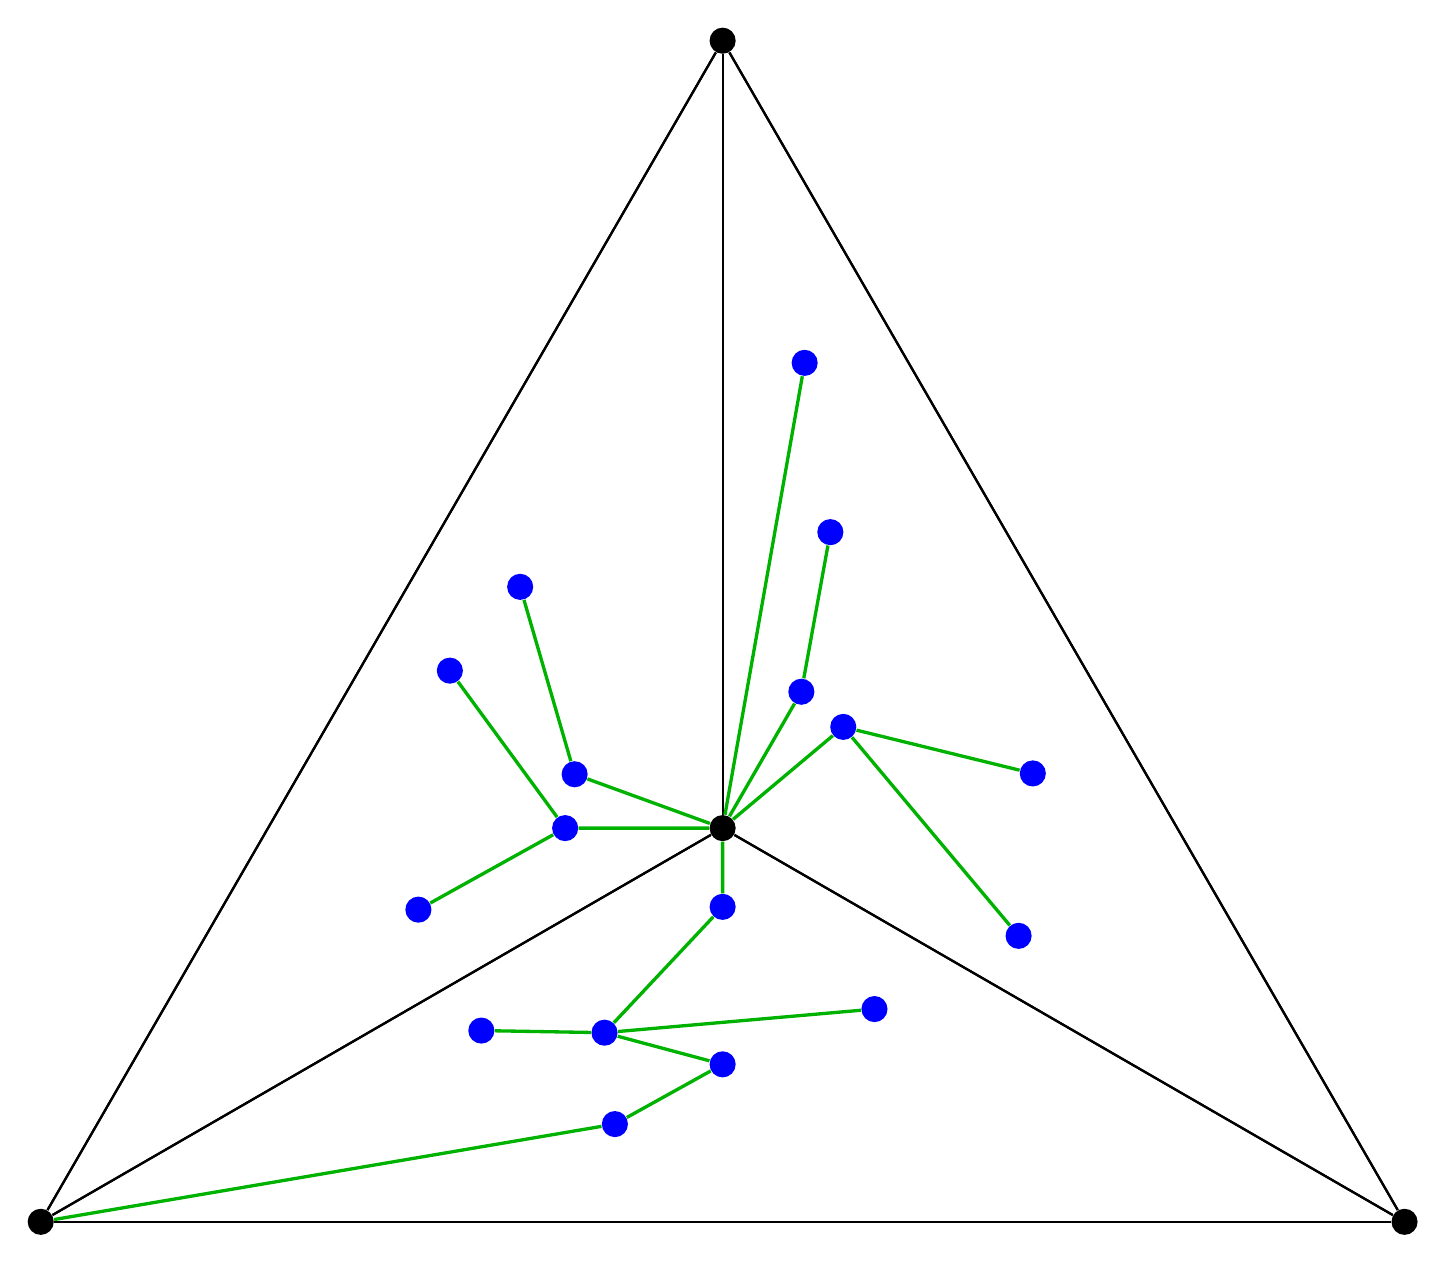
\begin{tikzpicture}[scale = 2]
    \foreach \angle in {0,...,2} {
        \node[fill, circle] (shell\angle) at (90+\angle*120:5) {};
    }
    \node[fill,circle] (shell3) at (0,0) {};
    \foreach \i in {0,...,3} {
        \foreach \j in {0,...,3} {
            \draw[thick] (shell\i) -- (shell\j);
        }
    }

    \node[fill, circle, \clrone] (1) at (-30-60:.5) {};
    \node[fill, circle, \clrone] (2) at (-30-90:1.5) {};
    \node[fill, circle, \clrone] (3) at (-30-20:1.5) {};
    \node[fill, circle, \clrone] (4) at (-30-60:1.5) {};
    \node[fill, circle, \clrone] (5) at (-30-80:2) {};
    \node[fill, circle, \clrone] (6) at (-30-110:2) {};
    
    \node[fill, circle, \clrone] (7) at (210-30:1) {};
    \node[fill, circle, \clrone] (8) at (210-50:1) {};
    \node[fill, circle, \clrone] (9) at (210-15:2) {};
    \node[fill, circle, \clrone] (10) at (210-60:2) {};
    \node[fill, circle, \clrone] (11) at (210-80:2) {};
    
    \node[fill, circle, \clrone] (12) at (90-30:1) {};
    \node[fill, circle, \clrone] (13) at (90-50:1) {};
    \node[fill, circle, \clrone] (14) at (90-20:2) {};
    \node[fill, circle, \clrone] (15) at (90-10:3) {};
    \node[fill, circle, \clrone] (16) at (90-80:2) {};
    \node[fill, circle, \clrone] (17) at (90-110:2) {};

    \draw[very thick, \clrtwo] (shell3) -- (1) -- (2) -- (3) (2) -- (4) -- (5) (2) -- (6) (shell3) -- (7) -- (9) (7) -- (10) (shell3) -- (8) -- (11) (shell3) -- (12) -- (14) (shell3) -- (15) (shell3) -- (13) -- (16) (13) -- (17);

    \draw[very thick, \clrtwo] (5) -- (shell1);


\end{tikzpicture}   

\end{document}